%%**************************************************************
%% Bachelor Thesis 2018
%%
%% Autor: Tobias Rahloff
%%
%%**************************************************************

%!TEX root = ../main.tex

%
% Nahezu alle Einstellungen koennen hier getaetigt werden
%

\RequirePackage[l2tabu, orthodox]{nag}	% weist in Commandozeile bzw. log auf veraltete LaTeX Syntax hin

\documentclass[%
	pdftex,
	oneside,			% Einseitiger Druck.
	12pt,				% Schriftgroesse
	parskip=half,		% Halbe Zeile Abstand zwischen Absätzen.
%	topmargin = 10pt,	% Abstand Seitenrand (Std:1in) zu Kopfzeile [laut log: unused]
	headheight = 12pt,	% Höhe der Kopfzeile
%	headsep = 30pt,	% Abstand zwischen Kopfzeile und Text Body  [laut log: unused]
	headsepline,		% Linie nach Kopfzeile.
	footsepline,		% Linie vor Fusszeile.
	footheight = 16pt,	% Höhe der Fusszeile
	abstracton,		% Abstract Überschriften
	DIV=calc,		% Satzspiegel berechnen
	BCOR=8mm,		% Bindekorrektur links: 8mm
	headinclude=false,	% Kopfzeile nicht in den Satzspiegel einbeziehen
	footinclude=false,	% Fußzeile nicht in den Satzspiegel einbeziehen
	listof=totoc,		% Abbildungs-/ Tabellenverzeichnis im Inhaltsverzeichnis darstellen
	toc=bibliography,	% Literaturverzeichnis im Inhaltsverzeichnis darstellen
]{scrreprt}	% Koma-Script report-Klasse, fuer laengere Bachelorarbeiten alternativ auch: scrbook

% Einstellungen laden
\usepackage{xstring}
\usepackage[utf8]{inputenc}
\usepackage[T1]{fontenc}

\newcommand{\einstellung}[1]{%
  \expandafter\newcommand\csname #1\endcsname{}
  \expandafter\newcommand\csname setze#1\endcsname[1]{\expandafter\renewcommand\csname#1\endcsname{##1}}
}
\newcommand{\langstr}[1]{\einstellung{lang#1}}

\einstellung{matrikelnr}
\einstellung{titel}
\einstellung{kurs}
\einstellung{datumAbgabe}
\einstellung{firma}
\einstellung{firmenort}
\einstellung{abgabeort}
\einstellung{abschluss}
\einstellung{studiengang}
\einstellung{dhbw}
\einstellung{betreuer}
\einstellung{gutachter}
\einstellung{zeitraum}
\einstellung{arbeit}
\einstellung{autor}
\einstellung{sprache}
\einstellung{schriftart}
\einstellung{seitenrand}
\einstellung{kapitelabstand}
\einstellung{spaltenabstand}
\einstellung{zeilenabstand}
\einstellung{zitierstil}
 % verfügbare Einstellungen
%%%%%%%%%%%%%%%%%%%%%%%%%%%%%%%%%%%%%%%%%%%%%%%%%%%%%%%%%%%%%%%%%%%%%%%%%%%%%%%
%                                   Einstellungen
%
% Hier können alle relevanten Einstellungen für diese Arbeit gesetzt werden.
% Dazu gehören Angaben u.a. über den Autor sowie Formatierungen.
%
%
%%%%%%%%%%%%%%%%%%%%%%%%%%%%%%%%%%%%%%%%%%%%%%%%%%%%%%%%%%%%%%%%%%%%%%%%%%%%%%%


%%%%%%%%%%%%%%%%%%%%%%%%%%%%%%%%%%%% Sprache %%%%%%%%%%%%%%%%%%%%%%%%%%%%%%%%%%%
%% Aktuell sind Deutsch und Englisch unterstützt.
%% Es werden nicht nur alle vom Dokument erzeugten Texte in
%% der entsprechenden Sprache angezeigt, sondern auch weitere
%% Aspekte angepasst, wie z.B. die Anführungszeichen und
%% Datumsformate.
\setzesprache{en} % oder en
%%%%%%%%%%%%%%%%%%%%%%%%%%%%%%%%%%%%%%%%%%%%%%%%%%%%%%%%%%%%%%%%%%%%%%%%%%%%%%%%

%%%%%%%%%%%%%%%%%%%%%%%%%%%%%%%%%%% Angaben  %%%%%%%%%%%%%%%%%%%%%%%%%%%%%%%%%%%
%% Die meisten der folgenden Daten werden auf dem
%% Deckblatt angezeigt, einige auch im weiteren Verlauf
%% des Dokuments.
\setzematrikelnr{1234510}
\setzekurs{ABC2008DE}
\setzetitel{In der Regel haben wir einen zweizeiligen Bachelorthesistitel}
\setzedatumAbgabe{August 2011}
\setzefirma{Firma GmbH}
\setzefirmenort{Firmenort}
\setzeabgabeort{Abgabeort}
\setzeabschluss{Bachelor of Engineering}
\setzestudiengang{Vorderasiatische Archäologie}
\setzedhbw{Karlsruhe}
\setzebetreuer{Dipl.-Ing.~(FH) Peter Pan}
\setzegutachter{Dr.\ Silvana Koch-Mehrin}
\setzezeitraum{12 Wochen}
\setzearbeit{Bachelorarbeit}
\setzeautor{Vorname Nachname}
%%%%%%%%%%%%%%%%%%%%%%%%%%%%%%%%%%%%%%%%%%%%%%%%%%%%%%%%%%%%%%%%%%%%%%%%%%%%%%%%

%%%%%%%%%%%%%%%%%%%%%%%%%%%% Literaturverzeichnis %%%%%%%%%%%%%%%%%%%%%%%%%%%%%%
%% Bei Fehlern während der Verarbeitung bitte in ads/header.tex bei der
%% Einbindung des Pakets biblatex (ungefähr ab Zeile 110,
%% einmal für jede Sprache), biber in bibtex ändern.
\newcommand{\ladeliteratur}{%
\addbibresource{bibliographie.bib}
\addbibresource{mendeley.bib}
}
%% Zitierstil
%% siehe: https://www.sharelatex.com/learn/Biblatex_citation_styles
%% mögliche Werte z.B numeric-comp, alphabetic, authoryear
\setzezitierstil{authoryear-icomp}
%%%%%%%%%%%%%%%%%%%%%%%%%%%%%%%%%%%%%%%%%%%%%%%%%%%%%%%%%%%%%%%%%%%%%%%%%%%%%%%%

%%%%%%%%%%%%%%%%%%%%%%%%%%%%%%%%% Layout %%%%%%%%%%%%%%%%%%%%%%%%%%%%%%%%%%%%%%%
%% Verschiedene Schriftarten
\setzeschriftart{mathpazo} % palatino oder goudysans, lmodern, libertine

%% Paket um Textteile drehen zu können
%\usepackage{rotating}
%% Paket um Seite im Querformat anzuzeigen
%\usepackage{lscape}

%% Seitenränder
\setzeseitenrand{2.5cm}

%% Abstand vor Kapitelüberschriften zum oberen Seitenrand
\setzekapitelabstand{20pt}

%% Spaltenabstand
\setzespaltenabstand{10pt}
%%Zeilenabstand innerhalb einer Tabelle
\setzezeilenabstand{1.5}
%%%%%%%%%%%%%%%%%%%%%%%%%%%%%%%%%%%%%%%%%%%%%%%%%%%%%%%%%%%%%%%%%%%%%%%%%%%%%%%%

%%%%%%%%%%%%%%%%%%%%%%%%%%%%% Verschiedenes  %%%%%%%%%%%%%%%%%%%%%%%%%%%%%%%%%%%
%% Farben (Angabe in HTML-Notation mit großen Buchstaben)
\newcommand{\ladefarben}{%
	\definecolor{LinkColor}{HTML}{3B5998}
	\definecolor{ListingBackground}{HTML}{FCF7DE}
}
%% Mathematikpakete benutzen (Pakete aktivieren)
%\usepackage{amsmath}
%\usepackage{amssymb}

%% Programmiersprachen Highlighting (Listings)
\newcommand{\listingsettings}{%
	\lstset{%
		language=Java,			% Standardsprache des Quellcodes
		numbers=left,			% Zeilennummern links
		stepnumber=1,			% Jede Zeile nummerieren.
		numbersep=5pt,			% 5pt Abstand zum Quellcode
		numberstyle=\tiny,		% Zeichengrösse 'tiny' für die Nummern.
		breaklines=true,		% Zeilen umbrechen wenn notwendig.
		breakautoindent=true,	% Nach dem Zeilenumbruch Zeile einrücken.
		postbreak=\space,		% Bei Leerzeichen umbrechen.
		tabsize=2,				% Tabulatorgrösse 2
		basicstyle=\ttfamily\footnotesize, % Nichtproportionale Schrift, klein für den Quellcode
		showspaces=false,		% Leerzeichen nicht anzeigen.
		showstringspaces=false,	% Leerzeichen auch in Strings ('') nicht anzeigen.
		extendedchars=true,		% Alle Zeichen vom Latin1 Zeichensatz anzeigen.
		captionpos=b,			% sets the caption-position to bottom
		backgroundcolor=\color{ListingBackground}, % Hintergrundfarbe des Quellcodes setzen.
		xleftmargin=0pt,		% Rand links
		xrightmargin=0pt,		% Rand rechts
		frame=single,			% Rahmen an
		frameround=ffff,
		rulecolor=\color{darkgray},	% Rahmenfarbe
		fillcolor=\color{ListingBackground},
		keywordstyle=\color[rgb]{0.133,0.133,0.6},
		commentstyle=\color[rgb]{0.133,0.545,0.133},
		stringstyle=\color[rgb]{0.627,0.126,0.941}
	}
}
%%%%%%%%%%%%%%%%%%%%%%%%%%%%%%%%%%%%%%%%%%%%%%%%%%%%%%%%%%%%%%%%%%%%%%%%%%%%%%%%

%%%%%%%%%%%%%%%%%%%%%%%%%%%%%%%% Eigenes %%%%%%%%%%%%%%%%%%%%%%%%%%%%%%%%%%%%%%%
%% Hier können Ergänzungen zur Präambel vorgenommen werden (eigene Pakete, Einstellungen)



 % lese Einstellungen

\newcommand{\iflang}[2]{%
  \IfStrEq{\sprache}{#1}{#2}{}
}

\langstr{abkverz}
\langstr{anhang}
\langstr{glossar}
\langstr{deckblattabschlusshinleitung}
\langstr{artikelstudiengang}
\langstr{studiengang}
\langstr{anderdh}
\langstr{von}
\langstr{dbbearbeitungszeit}
\langstr{dbmatriknr}
\langstr{dbkurs}
\langstr{dbfirma}
\langstr{dbbetreuer}
\langstr{dbgutachter}
\langstr{sperrvermerk}
\langstr{erklaerung}
\langstr{abstract}
\langstr{listingname}
\langstr{listlistingname}
\langstr{listingautorefname}
 % verfügbare Strings
\input{lang/\sprache} % Übersetzung einlesen

% Einstellung der Sprache des Paketes Babel und der Verzeichnisüberschriften
\iflang{de}{\usepackage[english, ngerman]{babel}}
\iflang{en}{\usepackage[ngerman, english]{babel}} 


%%%%%%% Package Includes %%%%%%%

\usepackage[margin=\seitenrand,foot=1cm]{geometry}	% Seitenränder und Abstände
\usepackage[activate]{microtype} %Zeilenumbruch und mehr
\usepackage[onehalfspacing]{setspace}
\usepackage{makeidx}
\usepackage[autostyle=true,german=quotes]{csquotes}
\usepackage{longtable}
\usepackage{enumitem}	% mehr Optionen bei Aufzählungen
\usepackage{graphicx}
\usepackage{pdfpages}   % zum Einbinden von PDFs
\usepackage{xcolor} 	% für HTML-Notation
\usepackage{float}
\usepackage{array}
\usepackage{calc}		% zum Rechnen (Bildtabelle in Deckblatt)
\usepackage[right]{eurosym}
\usepackage{wrapfig}
\usepackage{pgffor} % für automatische Kapiteldateieinbindung
\usepackage[perpage, hang, multiple, stable]{footmisc} % Fussnoten
\usepackage[printonlyused]{acronym} % falls gewünscht kann die Option footnote eingefügt werden, dann wird die Erklärung nicht inline sondern in einer Fußnote dargestellt
\usepackage{listings}

% Notizen. Einsatz mit \todo{Notiz} oder \todo[inline]{Notiz}. 
\usepackage[obeyFinal,backgroundcolor=yellow,linecolor=black]{todonotes}
% Alle Notizen ausblenden mit der Option "final" in \documentclass[...] oder durch das auskommentieren folgender Zeile
% \usepackage[disable]{todonotes}

% Kommentarumgebung. Einsatz mit \comment{}. Alle Kommentare ausblenden mit dem Auskommentieren der folgenden und dem aktivieren der nächsten Zeile.
\newcommand{\comment}[1]{\par {\bfseries \color{blue} #1 \par}} %Kommentar anzeigen
% \newcommand{\comment}[1]{} %Kommentar ausblenden


%%%%%% Configuration %%%%%

%% Anwenden der Einstellungen

\usepackage{\schriftart}
\ladefarben{}

\usepackage{pgfplots}
\pgfplotsset{compat=1.15}

% Titel, Autor und Datum
\title{\titel}
\author{\autor}
\date{\datum}

% PDF Einstellungen
\usepackage[%
	pdftitle={\titel},
	pdfauthor={\autor},
	pdfsubject={\arbeit},
	pdfcreator={pdflatex, LaTeX with KOMA-Script},
	pdfpagemode=UseOutlines, 		% Beim Oeffnen Inhaltsverzeichnis anzeigen
	pdfdisplaydoctitle=true, 		% Dokumenttitel statt Dateiname anzeigen.
	pdflang={\sprache}, 			% Sprache des Dokuments.
]{hyperref}

% (Farb-)einstellungen für die Links im PDF
\hypersetup{%
	colorlinks=true, 		% Aktivieren von farbigen Links im Dokument
	linkcolor=LinkColor, 	% Farbe festlegen
	citecolor=LinkColor,
	filecolor=LinkColor,
	menucolor=LinkColor,
	urlcolor=LinkColor,
	linktocpage=true, 		% Nicht der Text sondern die Seitenzahlen in Verzeichnissen klickbar
	bookmarksnumbered=true 	% Überschriftsnummerierung im PDF Inhalt anzeigen.
}
% Workaround um Fehler in Hyperref, muss hier stehen bleiben
\usepackage{bookmark} %nur ein latex-Durchlauf für die Aktualisierung von Verzeichnissen nötig

% Schriftart in Captions etwas kleiner
\addtokomafont{caption}{\small}

% Literaturverweise (sowohl deutsch als auch englisch)
\iflang{de}{%
\usepackage[
	backend=biber,		% empfohlen. Falls biber Probleme macht: bibtex
	bibwarn=true,
	bibencoding=utf8,	% wenn .bib in utf8, sonst ascii
	sortlocale=de_DE,
	style=\zitierstil,
	citestyle=\citestyle,
]{biblatex}
}
\iflang{en}{%
\usepackage[
	backend=biber,		% empfohlen. Falls biber Probleme macht: bibtex
	bibwarn=true,
	bibencoding=utf8,	% wenn .bib in utf8, sonst ascii
	sortlocale=en_US,
	style=\zitierstil,
	citestyle=\citestyle,
]{biblatex}
}
% Custom Workaround for Baumgart-Style (Author, Title, Year) 
\usepackage{xpatch}
\usepackage{chngcntr}
\xapptobibmacro{cite}{\setunit{\nametitledelim}\printfield{year}}{}{}
\counterwithout{footnote}{chapter}

\ladeliteratur{}

% Glossar
\usepackage[nonumberlist,toc]{glossaries}

%%%%%% Additional settings %%%%%%

% Hurenkinder und Schusterjungen verhindern
% http://projekte.dante.de/DanteFAQ/Silbentrennung
\clubpenalty = 10000 % schließt Schusterjungen aus (Seitenumbruch nach der ersten Zeile eines neuen Absatzes)
\widowpenalty = 10000 % schließt Hurenkinder aus (die letzte Zeile eines Absatzes steht auf einer neuen Seite)
\displaywidowpenalty=10000

% Bildpfad
\graphicspath{{images/}}

% Einige häufig verwendete Sprachen
\lstloadlanguages{PHP,Python,Java,C,C++,bash}
\listingsettings{}
% Umbennung des Listings
\renewcommand\lstlistingname{\langlistingname}
\renewcommand\lstlistlistingname{\langlistlistingname}
\def\lstlistingautorefname{\langlistingautorefname}

% Abstände in Tabellen
\setlength{\tabcolsep}{\spaltenabstand}
\renewcommand{\arraystretch}{\zeilenabstand}


% \makeglossaries
% %!TEX root = ../main.tex

%
% vorher in Konsole folgendes aufrufen:
%	makeglossaries makeglossaries dokumentation.acn && makeglossaries dokumentation.glo
%

%
% Glossareintraege --> referenz, name, beschreibung
% Aufruf mit \gls{...}
%
\newglossaryentry{Glossareintrag}{name={Glossareintrag},plural={Glossareinträge},description={Ein Glossar beschreibt verschiedenste Dinge in kurzen Worten}}

% \printglossary[type=\acronymtype,style=long]

\begin{document}

	% Deckblatt
	\begin{spacing}{1}
		%!TEX root = ../main.tex

\begin{titlepage}
	\begin{longtable}{p{8.2cm} p{5.4cm}}
		{\raisebox{\ht\strutbox-\totalheight}{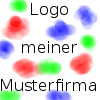
\includegraphics{images/misc/firma-deckblatt.png}}} &
		{\raisebox{\ht\strutbox-\totalheight}{
\includegraphics[height=2.5cm]{images/misc/dhbw.png}}}
	\end{longtable}
	\enlargethispage{20mm}
	\begin{center}
		\vspace*{12mm}	{\LARGE\textbf \titel }\\
		\vspace*{12mm}	{\large\textbf \arbeit}\\
		\vspace*{12mm}	\langdeckblattabschlusshinleitung\\
		\vspace*{3mm}		{\textbf \abschluss}\\
		\vspace*{12mm}	\langartikelstudiengang{} \langstudiengang{} \studiengang\\
    \vspace*{3mm}		\langanderdh{} \dhbw\\
		\vspace*{12mm}	\langvon\\
		\vspace*{3mm}		{\large\textbf \autor}\\
		\vspace*{12mm}	\datumAbgabe\\
	\end{center}
	\vfill
	\begin{spacing}{1.2}
	\begin{tabbing}
		mmmmmmmmmmmmmmmmmmmmmmmmmm             \= \kill
		\textbf{\langdbbearbeitungszeit}       \>  \zeitraum\\
		\textbf{\langdbmatriknr, \langdbkurs}  \>  \matrikelnr, \kurs\\
		\textbf{\langdbfirma}                  \>  \firma, \firmenort\\
		\textbf{\langdbbetreuer}               \>  \betreuer\\
		\textbf{\langdbgutachter}              \>  \gutachter
	\end{tabbing}
	\end{spacing}
\end{titlepage}

	\end{spacing}
	\newpage

	\pagenumbering{Roman}

	% Sperrvermerk
% 	%!TEX root = ../main.tex

\thispagestyle{empty}
% Sperrvermerk direkt hinter Titelseite
\section*{\langsperrvermerk}

\vspace*{2em}

\iflang{de}{%
  Die vorliegende {\arbeit} mit dem Titel {\itshape{} \titel{}\/} enthält unternehmensinterne bzw. vertrauliche Informationen der {\firma}, ist deshalb mit einem Sperrvermerk versehen und wird ausschließlich zu Prüfungszwecken am Studiengang {\studiengang} der Dualen Hochschule Baden-Württemberg {\dhbw} vorgelegt. Sie ist ausschließlich zur Einsicht durch den zugeteilten Gutachter, die Leitung des Studiengangs und ggf. den Prüfungsausschuss des Studiengangs bestimmt.  Es ist untersagt,
  \begin{itemize}
  \item den Inhalt dieser Arbeit (einschließlich Daten, Abbildungen, Tabellen, Zeichnungen usw.) als Ganzes oder auszugsweise weiterzugeben,
  \item Kopien oder Abschriften dieser Arbeit (einschließlich Daten, Abbildungen, Tabellen, Zeichnungen usw.) als Ganzes oder in Auszügen anzufertigen,
  \item diese Arbeit zu veröffentlichen bzw. digital, elektronisch oder virtuell zur Verfügung zu stellen. 
  \end{itemize}
Jede anderweitige Einsichtnahme und Veröffentlichung – auch von Teilen der Arbeit – bedarf der vorherigen Zustimmung durch den Verfasser und {\firma}.
}

%http://www.ib.dhbw-mannheim.de/fileadmin/ms/bwl-ib/Downloads_alt/Leitfaden_31.05.pdf

\iflang{en}{%
  The {\arbeit} on hand 
  \begin{center}{\itshape{} \titel{}\/}\end{center} 
   contains internal resp.\ confidential data of {\firma}. It is intended solely for inspection by the assigned examiner, the head of the {\studiengang} department and, if necessary, the Audit Committee \langanderdh{} {\dhbw}. It is strictly forbidden
    \begin{itemize}
    \item to distribute the content of this paper (including data, figures, tables, charts etc.) as a whole or in extracts,
    \item to make copies or transcripts of this paper or of parts of it,
    \item to display this paper or make it available in digital, electronic or virtual form.
    \end{itemize}
  Exceptional cases may be considered through permission granted in written form by the author and {\firma}.
}

\vspace{3em}

\abgabeort, \datumAbgabe
\vspace{4em}

\rule{6cm}{0.4pt}\\
\autor

% 	\newpage

	% Abstract
	%!TEX root = ../main.tex

\pagestyle{empty}

\iflang{de}{%
% Dieser deutsche Teil wird nur angezeigt, wenn die Sprache auf Deutsch eingestellt ist.
\renewcommand{\abstractname}{\langabstract} % Text für Überschrift

% \begin{otherlanguage}{english} % auskommentieren, wenn Abstract auf Deutsch sein soll
\begin{abstract}
Abstract normalerweise auf Englisch. Siehe:  \url{http://www.dhbw.de/fileadmin/user/public/Dokumente/Portal/Richtlinien_Praxismodule_Studien_und_Bachelorarbeiten_JG2011ff.pdf} (8.3.1 Inhaltsverzeichnis)

Ein "`Abstract"' ist eine prägnante Inhaltsangabe, ein Abriss ohne Interpretation und Wertung einer wissenschaftlichen Arbeit. In DIN 1426 wird das (oder auch der) Abstract als Kurzreferat zur Inhaltsangabe beschrieben.

\begin{description}
\item[Objektivität] soll sich jeder persönlichen Wertung enthalten
\item[Kürze] soll so kurz wie möglich sein
\item[Genauigkeit] soll genau die Inhalte und die Meinung der Originalarbeit wiedergeben
\end{description}

Üblicherweise müssen wissenschaftliche Artikel einen Abstract enthalten, typischerweise von 100-150 Wörtern, ohne Bilder und Literaturzitate und in einem Absatz.

Quelle: \url{http://de.wikipedia.org/wiki/Abstract} Abgerufen 07.07.2011

Diese etwa einseitige Zusammenfassung soll es dem Leser ermöglichen, Inhalt der Arbeit und Vorgehensweise
des Autors rasch zu überblicken. Gegenstand des Abstract sind insbesondere 
\begin{itemize}
\item Problemstellung der Arbeit,
\item im Rahmen der Arbeit geprüfte Hypothesen bzw. beantwortete Fragen,
\item der Analyse zugrunde liegende Methode,
\item wesentliche, im Rahmen der Arbeit gewonnene Erkenntnisse,
\item Einschränkungen des Gültigkeitsbereichs (der Erkenntnisse) sowie nicht beantwortete Fragen. 
\end{itemize}
Quelle: \url{http://www.ib.dhbw-mannheim.de/fileadmin/ms/bwl-ib/Downloads_alt/Leitfaden_31.05.pdf}, S.~49
\end{abstract}
% \end{otherlanguage} % auskommentieren, wenn Abstract auf Deutsch sein soll
}



\iflang{en}{%
% Dieser englische Teil wird nur angezeigt, wenn die Sprache auf Englisch eingestellt ist.
\renewcommand{\abstractname}{\langabstract} % Text für Überschrift

\begin{abstract}
An abstract is a brief summary of a research article, thesis, review, conference proceeding or any in-depth analysis of a particular subject or discipline, and is often used to help the reader quickly ascertain the paper's purpose. When used, an abstract always appears at the beginning of a manuscript, acting as the point-of-entry for any given scientific paper or patent application. Abstracting and indexing services for various academic disciplines are aimed at compiling a body of literature for that particular subject.

The terms précis or synopsis are used in some publications to refer to the same thing that other publications might call an ``abstract''. In ``management'' reports, an executive summary usually contains more information (and often more sensitive information) than the abstract does.

Quelle: \url{http://en.wikipedia.org/wiki/Abstract_(summary)}

\end{abstract}
}
	\newpage
	
	
	\pagenumbering{Roman}

	% Abkürzungsverzeichnis
	\cleardoublepage
	%!TEX root = ../main.tex

\addchap{\langabkverz}
%nur verwendete Akronyme werden letztlich im Abkürzungsverzeichnis des Dokuments angezeigt
%Verwendung: 
%		\ac{Abk.}   --> fügt die Abkürzung ein, beim ersten Aufruf wird zusätzlich automatisch die ausgeschriebene Version davor eingefügt bzw. in einer Fußnote (hierfür muss in header.tex \usepackage[printonlyused,footnote]{acronym} stehen) dargestellt
%		\acs{Abk.}   -->  fügt die Abkürzung ein
%		\acf{Abk.}   --> fügt die Abkürzung UND die Erklärung ein
%		\acl{Abk.}   --> fügt nur die Erklärung ein
%		\acp{Abk.}  --> gibt Plural aus (angefügtes 's'); das zusätzliche 'p' funktioniert auch bei obigen Befehlen
%	siehe auch: http://golatex.de/wiki/%5Cacronym
%	
\begin{acronym}[YTMMM]
\setlength{\itemsep}{-\parsep}

\acro{AGPL}{Affero GNU General Public License}
\acro{WSN}{Wireless Sensor Network}
\acro{MANET}{Mobile wireless Ad-hoc NETwork}
\acro{MAC}{Multiple Access Control}
\acro{QoS}{Quality of Service}
\acro{DSR}{Dynamic Source Routing}
\acro{API}{Application Programming Interface}
\acro{WYSIWYG}{What You See Is What You Get}
\acro{HTML}{HyperText Markup Language}
\acro{PaaS}{Platform-as-a-Service}
\acro{ESP}{Event Stream Processing}
\acro{ESB}{Enterprise Service Bus}
\end{acronym}


	% Abbildungsverzeichnis
	\cleardoublepage
	\listoffigures

	%Tabellenverzeichnis
	\cleardoublepage
	\listoftables

	% Quellcodeverzeichnis
	\cleardoublepage
	\lstlistoflistings
	\cleardoublepage


	\pagestyle{plain}		% nur Seitenzahlen im Fuß
	
	\RedeclareSectionCommand[beforeskip=\kapitelabstand         ]{chapter} % stellt Abstand vor Kapitelüberschriften ein

	% Inhaltsverzeichnis
	\begin{spacing}{1.1}
		\begingroup
		
			% auskommentieren für Seitenzahlen unter Inhaltsverzeichnis
			\renewcommand*{\chapterpagestyle}{empty}
			\pagestyle{empty}
			
			
			\setcounter{tocdepth}{10}
			%für die Anzeige von Unterkapiteln im Inhaltsverzeichnis
			%\setcounter{tocdepth}{2}
			
			\tableofcontents
			\clearpage
		\endgroup
	\end{spacing}
	\newpage

	\pagenumbering{arabic}
	
	\pagestyle{headings}		% Kolumnentitel im Kopf, Seitenzahlen im Fuß

	% Examples
    % %!TEX root = ../main.tex

\chapter{Das erste Kapitel}
Erste Erwähnung eines Akronyms wird als Fußnote angezeigt. Jede weitere wird
nur verlinkt: \acf{AGPL}. \cite{fsf:2007}

Verweise auf das Glossar: \gls{Glossareintrag}, \glspl{Glossareintrag}

Nur erwähnte Literaturverweise werden auch im Literaturverzeichnis gedruckt:
\cite{baumgartner:2002}, \cite{dreyfus:1980}

Meine erste Fußnote\footnote{Ich bin eine Fußnote} asdasd.

Meine zweite Fußnote\footnotemark

\begin{wrapfigure}{r}{.4\textwidth}

\includegraphics[width=\linewidth]{images/misc/logo.png}
\vspace{-15pt}
\caption{Das Logo der Musterfirma\footnotemark}
\end{wrapfigure}
%Quelle muss in Fußnote stehen (da sonst aufgrund eines Fehlers nicht kompiliert
% wird)
Looking for the one superhero comic you just have to read. Following the antics and adventures of May Mayday Parker, this Spider-book has everything you could want in a comic--action, laughs, mystery and someone in a Spidey suit. Collects Alias \#1-28, What If. Jessica Jones had Joined the Avengers. In her inaugural arc, Jessicas life immediately becomes expendable when she uncovers the potentially explosive secret of one heros true identity. In her inaugural arc, Jessicas life immediately becomes expendable when she uncovers the potentially explosive secret of one heros true identity.

Once upon a time, Jessica Jones was a costumed super-hero, just not a very good one. First, a story where Wolverine and Hulk come together, and then Captain America and Cable meet up. In a city of Marvels, Jessica Jones never found her niche. The classic adventures of Spider-Man from the early days up until the 90s. Looking for the one superhero comic you just have to read. In her inaugural arc, Jessicas life immediately becomes expendable when she uncovers the potentially explosive secret of one heros true identity.



\footnotetext{aus \cite{mustermann:2012}}
    % %!TEX root = ../main.tex

\chapter{Beispiel Code-schnipsel einbinden}

%title wird unter dem Bsp. abgedruckt
%caption wird im Verzeichnis abgedruckt
%label wird zum referenzieren benutzt, muss einzigartig sein.

\begin{lstlisting}[caption=Code-Beispiel, label=Bsp.1]
public class HelloWorld {
	public static void main (String[] args) {
		// Ausgabe Hello World!
		System.out.println("Hello World!");
	}
}
\end{lstlisting}

%language ändert die Sprache. (Wenn nur eine Sprache verwendet wird, kann diese Sprache in einstellungen.tex geändert werden. Standardmäßig Java.)
\begin{lstlisting}[caption=Python-Code, label=Python-Code, title=Titel des Python-Codes,language=Python]
def quicksort(liste):
if len(liste) <= 1:
	return liste
pivotelement = liste.pop()
links = [element for element in liste if element < pivotelement]
rechts = [element for element in liste if element >= pivotelement]
return quicksort(links) + [pivotelement] + quicksort(rechts)
# Quelle: http://de.wikipedia.org/wiki/Python_(Programmiersprache)
\end{lstlisting}

\section{lorem ipsum}
Looking for the one superhero comic you just have to read. Following the antics and adventures of May Mayday Parker, this Spider-book has everything you could want in a comic--action, laughs, mystery and someone in a Spidey suit. Collects Alias \#1-28, What If. Jessica Jones had Joined the Avengers. In her inaugural arc, Jessicas life immediately becomes expendable when she uncovers the potentially explosive secret of one heros true identity. 

Once upon a time, Jessica Jones was a costumed super-hero, just not a very good one. First, a story where Wolverine and Hulk come together, and then Captain America and Cable meet up. In a city of Marvels, Jessica Jones never found her niche. The classic adventures of Spider-Man from the early days up until the 90s. Looking for the one superhero comic you just have to read.

Meet all of Spideys deadly enemies, from the Green Goblin and Doctor Octopus to Venom and Carnage, plus see Peter Parker fall in love, face tragedy and triumph, and learn that with great power comes great responsibility. In a city of Marvels, Jessica Jones never found her niche. Bitten by a radioactive spider, high school student Peter Parker gained the speed, strength and powers of a spider. Looking for the one superhero comic you just have to read. What do you get when you ask the question, What if Spider-Man had a daughter.

The classic adventures of Spider-Man from the early days up until the 90s. Amazing Spider-Man is the cornerstone of the Marvel Universe. But will each partner’s combined strength be enough. Adopting the name Spider-Man, Peter hoped to start a career using his new abilities. Youve found it.

\section{Verweis auf Code}
Verweis auf den Code \autoref{Bsp.1}.\\
und der Python-Code \autoref{Python-Code}.

Zweite Erwähnung einer Abkürzung \ac{AGPL} (Erlärung wird nicht mehr angezeigt)
	
	% Inhalt
% 	\chapter{Introduction}


\section{Problem Definition}

Stream-processing has become one of the major computing problems enterprise system architects face today. Due to recent trends such as IoT, the amount of data that has to be categorized, analyzed and processed skyrocketed. 
Many companies such as Netflix\footnote{\url{https://aws.amazon.com/solutions/case-studies/netflix-kinesis-streams/}} or Uber\footnote{\url{https://flink.apache.org/poweredby}} adopted stream-processing patterns in combination with serverless computing to take on challenges that demand highly scale able and performant systems. 
This approach is particularly favourable for companies that deliver IoT solutions such as Toyota\footnote{\url{https://aws.amazon.com/solutions/case-studies/toyota-tsusho/}} or Quest\footnote{\url{https://customers.microsoft.com/en-us/story/quest}}.
\section{Objective and Problem Statement}

The purpose of this research is to develop a framework for architects that enables them to decide if a "serverless" architectural approach is fitted for their stream-processing use-case.
One major objective is to asses the current industry understanding of "serverless" and evaluate the viability and range of application of this architecture pattern.
Moreover, it is supposed to assist the process of highlevel system design by providing a reference and guidance by introducing fPaaS\footnote{"Function-Platform-as-a-Service". Defined by Gartner \autocite{Chandrasekaran2017EvolutionWhen}} capabilities and caveats. 


\section{Scope}

UseCase: StreamProcessing.

\begin{figure}[ht]
    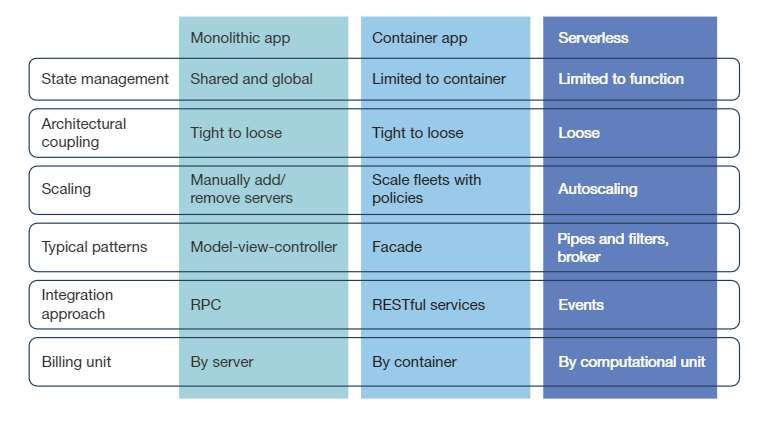
\includegraphics[width=\linewidth]{images/serverless/demyst.png}\centering
    \caption{\cite{Hammond2018DemystifyingComputing}}
\end{figure}
\section{Importance and Significance of the Study}

No TTF papers on the topic

no real comparison for streaming 
\section{Thesis Content}

Within the following chapters, the presented research questions will be systematically addressed and answered. Hereby the thesis content is structured as follows:

\begin{center}
\begin{tabular}{ | m{11em} | p{23em}| } 
\hline
 \textbf{Research Method} & 
 The applied research model, the operationalization approach, research deliverables, design principles and result evaluation.  \\
 \hline 
 
 \textbf{Theoretical Background} & 
 A general introduction into the cloud-computing domain and "Serverless" architectures, as well as a systematic literature review on both topics. \\
 \hline 
 
 \textbf{Design} & 
 whatev \\
 \hline 
 
 \textbf{Validation} & 
 Use case driven validation of method applicability and method usability by open source experts. \\
 \hline 
 
 \textbf{Discussion} & 
 Final research results, existing limitations, recommendation for future research, as well as an assessment of the practical value of the presented method. \\
 \hline 
 
 \textbf{Bibliography} & 
 Cited scientific literature throughout the thesis. \\
 \hline 
 
 \textbf{Appendices} & 
 Deliverables, too large or unsuitable to be placed within the main body of the research document. \\
\hline
\end{tabular}
\end{center}


% 	\chapter{Theoretical Background}

\section{Cloud Computing}

whatev
\section{Containerization}

whatev
\section{Stream Processing}
\section{"Serverless"}

whatev
% 	\chapter{Research Method}

\section{Method Evaluation}

TTF vs TAM vs UTAUT vs FVM ?

\begin{figure}[ht]
    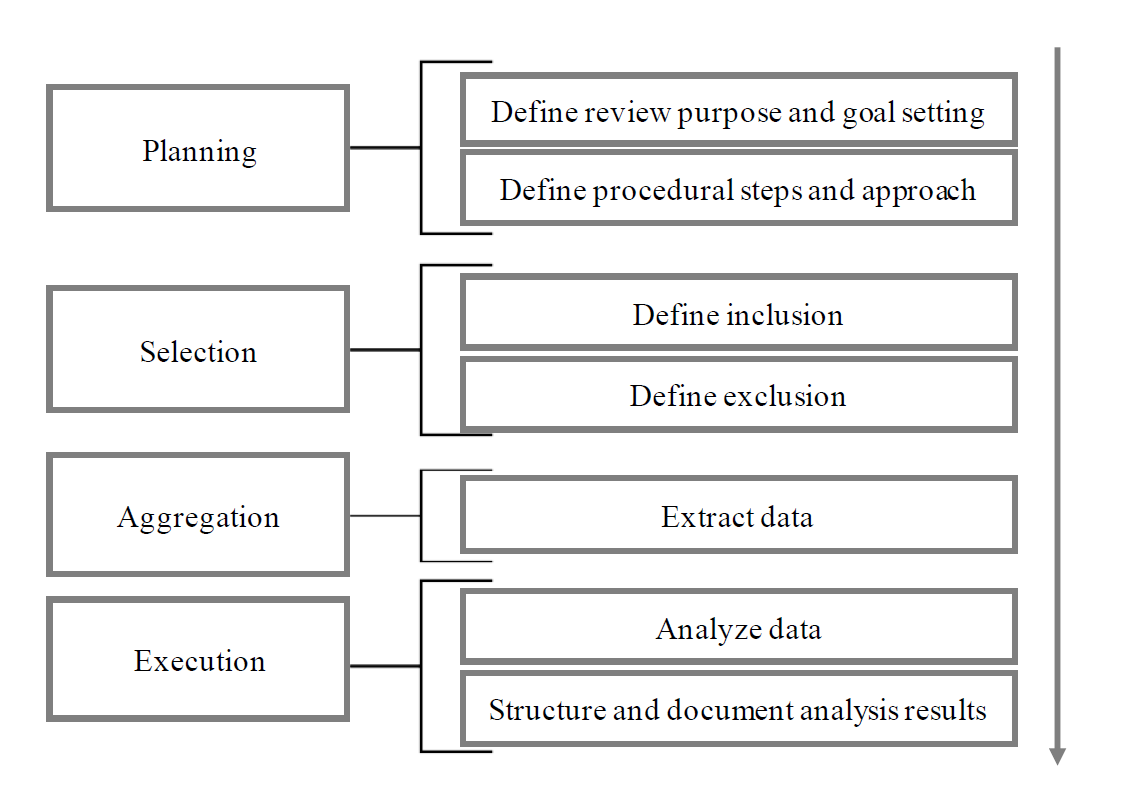
\includegraphics[width=0.8\linewidth]{images/methodology/litSearc.png}\centering
    \caption{\cite{Okoli2010AResearch}}
\end{figure}

\section{Research Model}


\begin{figure}[ht]
    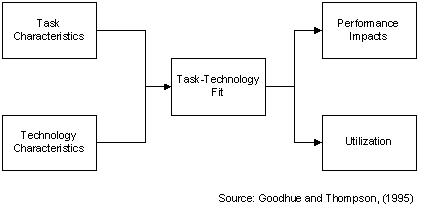
\includegraphics[width=0.7\linewidth]{images/methodology/ttf.jpg}\centering
    \caption{\cite{Goodhue1995Task-TechnologyPerformance}}
\end{figure}

\begin{enumerate}
    \item quality
    \item locatability
    \item authorization
    \item compatibility
    \item ease of use/training
    \item production timeliness
    \item systems reliability
    \item relationship with users
\end{enumerate}

\begin{figure}[ht]
    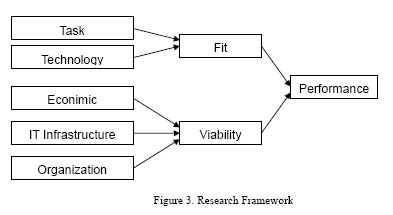
\includegraphics[width=0.7\linewidth]{images/methodology/fvm.jpg}\centering
    \caption{\cite{Liang2007AdoptionModel}}
\end{figure}
\section{Operationalization}

\url{https://explorable.com/operationalization}

% 	\chapter{Design}

desi
% 	\chapter{Validation}

\section{General Method Suitability}

Whatever, whatever.
\section{Method Applicability}

Whatever, whatever.
\section{Reliability}

Whatever, whatever.
\section{Validity}

Whatever, whatever.
% 	\chapter{Discussion \& Conclusion}

\section{Findings and Research Contribution}

findingsAndResearchContribution \cite{Dishaw1998SupportingAnalysis}
\section{General Conclusion}

generalConclusion
\section{Thesis Results}

Whatever, whatever.
\section{Scientific Relevance}

Whatever, whatever.
\section{Future Research}

Whatever, whatever.

	
	

\foreach \i in {00,01,02,03,04,05,06,07,08,09,...,99} {%
    \edef\FileName{content/\i chapter}%
    \IfFileExists{\FileName}{%
        \input{\FileName}
    }
    {%
    				%file does not exist
    }
}

	

	
    

	% Literaturverzeichnis
	\cleardoublepage
	\printbibliography

	
% 	sdonstiger Anhang
	\clearpage
	\appendix
	% !TeX root = ../main.tex

\addchap{\langanhang}

(Beispielhafter Anhang)
 

{\Large
\begin{enumerate}[label=\Alph*.]
	\item Assignment
	\item List of CD Contents
	\item CD 
\end{enumerate}
}
\pagebreak
%\includepdf[pages=-,scale=.9,pagecommand={}]{Aufgabenstellung.pdf} % PDF um 10% verkleinert einbinden --> Kopf- und Fußzeile  werden so korrekt dargestellt. Die Option `pages' ermöglicht es, eine bestimmte Sequenz von Seiten (z.B. 2-10 oder `-' für alle Seiten) auszuwählen.
\pagebreak
\section*{A. Kinesis Data Generator CloudFormation Template}\label{app:KDG}

    \begin{lstlisting}[language=json,firstnumber=1]
    {
      "AWSTemplateFormatVersion" : "2010-09-09",
      
      "Description" : "This template creates an Amazon Cognito User Pool and Identity Pool, with a single user.  It assigns a role to authenticated users in the identity pool to enable the users to use the Kinesis Data Generator tool.",
      
      "Parameters" : {
    
        "Username": {
          "Description": "The username of the user you want to create in Amazon Cognito.",
          "Type": "String",
          "AllowedPattern": "^(?=\\s*\\S).*\$",
          "ConstraintDescription": " cannot be empty"
    
        },
        "Password": {
          "Description": "The password of the user you want to create in Amazon Cognito.",
          "Type": "String",
          "NoEcho": true,
          "AllowedPattern": "^(?=.*[A-Za-z])(?=.*\\d)[A-Za-z\\d]{6,}\$",
          "ConstraintDescription": " must be at least 6 alpha-numeric characters, and contain at least one number"
        }
      },
      
      "Metadata": {
        "AWS::CloudFormation::Interface": {
          "ParameterGroups": [
            {
              "Label": {
                "default": "Cognito User for Kinesis Data Generator"
              },
              "Parameters": [
                "Username",
                "Password"
              ]
            }
          ]
        }
      },
      
      
      "Resources" : {
    
        "DataGenCognitoSetupLambdaFunc" : {
          "Type" : "AWS::Lambda::Function",
          "Properties" : {
            "Code": {
              "S3Bucket" : "kinesis-helpers",
              "S3Key": "datagen-cognito-setup.zip"
            },
            "Description": "Creates a Cognito User Pool, Identity Pool, and a User.  Returns IDs to be used in the Kinesis Data Generator.",
            "FunctionName": "KinesisDataGeneratorCognitoSetup",
            "Handler": "createCognitoPool.createPoolAndUser",
            "Role": { "Fn::GetAtt" : ["LambdaExecutionRole", "Arn"] },
            "Runtime": "nodejs4.3",
            "Timeout": 60
          }
        },
        
        "LambdaExecutionRole": {
          "Type": "AWS::IAM::Role",
          "Properties": {
            "AssumeRolePolicyDocument": {
              "Version": "2012-10-17",
              "Statement": [{ "Effect": "Allow", "Principal": {"Service": ["lambda.amazonaws.com"]}, "Action": ["sts:AssumeRole"] }]
            },
            "Path": "/",
            "Policies": [{
              "PolicyName": "root",
              "PolicyDocument": {
                "Version": "2012-10-17",
                "Statement": [
                  {
                    "Effect": "Allow",
                    "Action": ["logs:*"],
                    "Resource": "arn:aws:logs:*:*:*" },
                  {
                    "Effect": "Allow",
                    "Action": [
                      "cognito-idp:AdminConfirmSignUp",
                      "cognito-idp:CreateUserPoolClient",
                      "cognito-idp:AdminCreateUser"
                    ],
                    "Resource": [
                      "arn:aws:cognito-idp:*:*:userpool/*"
                    ]
                  },
                  {
                    "Effect": "Allow",
                    "Action": [
                      "cognito-idp:CreateUserPool",
                      "cognito-identity:*"
                    ],
                    "Resource": "*" },
                  {
                    "Effect": "Allow",
                    "Action": ["iam:UpdateAssumeRolePolicy"],
                    "Resource": [
                      {"Fn::GetAtt" : ["AuthenticatedUserRole", "Arn"] },
                      {"Fn::GetAtt" : ["UnauthenticatedUserRole", "Arn"] }
                    ]
                  },
                  {
                    "Effect": "Allow",
                    "Action": ["iam:PassRole"],
                    "Resource": [
                      {"Fn::GetAtt" : ["AuthenticatedUserRole", "Arn"] },
                      {"Fn::GetAtt" : ["UnauthenticatedUserRole", "Arn"] }
                    ]
                  }
                ]
              }
            }]
          }
        },
        
        "SetupCognitoCustom" : {
          "Type": "Custom::DataGenCognitoSetupLambdaFunc",
          "Properties": {
            "ServiceToken": { "Fn::GetAtt" : ["DataGenCognitoSetupLambdaFunc", "Arn"] },
            "Region": {"Ref": "AWS::Region"},
            "Username": {"Ref": "Username"},
            "Password": {"Ref": "Password"},
            "AuthRoleName": {"Ref": "AuthenticatedUserRole"},
            "AuthRoleArn": { "Fn::GetAtt" : ["AuthenticatedUserRole", "Arn"] },
            "UnauthRoleName": {"Ref": "UnauthenticatedUserRole"},
            "UnauthRoleArn": { "Fn::GetAtt" : ["UnauthenticatedUserRole", "Arn"] }
    
          }
        },
        
        "AuthenticatedUserRole": {
          "Type": "AWS::IAM::Role",
          "Properties": {
            "AssumeRolePolicyDocument": {
              "Version": "2012-10-17",
              "Statement": [{ "Effect": "Allow", "Principal": {"Federated": ["cognito-identity.amazonaws.com"]}, "Action": ["sts:AssumeRoleWithWebIdentity"] }]
            },
            "Path": "/",
            "Policies": [{
              "PolicyName": "root",
              "PolicyDocument": {
                "Version": "2012-10-17",
                "Statement": [
                  {
                    "Action": [
                      "kinesis:DescribeStream",
                      "kinesis:PutRecord",
                      "kinesis:PutRecords"
                    ],
                    "Resource": [
                      "arn:aws:kinesis:*:*:stream/*"
                    ],
                    "Effect": "Allow"
                  },
                  {
                    "Action": [
                      "firehose:DescribeDeliveryStream",
                      "firehose:PutRecord",
                      "firehose:PutRecordBatch"
                    ],
                    "Resource": [
                      "arn:aws:firehose:*:*:deliverystream/*"
                    ],
                    "Effect": "Allow"
                  },
                  {
                    "Action": [
                      "mobileanalytics:PutEvents",
                      "cognito-sync:*",
                      "cognito-identity:*",
                      "ec2:DescribeRegions",
                      "firehose:ListDeliveryStreams",
                      "kinesis:ListStreams"
                    ],
                    "Resource": [
                      "*"
                    ],
                    "Effect": "Allow"
                  }
                ]
              }
            }]
          }
        },
        
        "UnauthenticatedUserRole": {
          "Type": "AWS::IAM::Role",
          "Properties": {
            "AssumeRolePolicyDocument": {
              "Version": "2012-10-17",
              "Statement": [{ "Effect": "Allow", "Principal": {"Federated": ["cognito-identity.amazonaws.com"]}, "Action": ["sts:AssumeRoleWithWebIdentity"] }]
            },
            "Path": "/",
            "Policies": [{
              "PolicyName": "root",
              "PolicyDocument": {
                "Version": "2012-10-17",
                "Statement": [
                  {
                    "Effect": "Allow",
                    "Action": [
                      "mobileanalytics:PutEvents",
                      "cognito-sync:*"
                    ],
                    "Resource": [
                      "*"
                    ]
                  }
                ]
              }
            }]
          }
        }
      },
      
      "Outputs":{
        "KinesisDataGeneratorUrl": {
          "Description": "The URL for your Kinesis Data Generator.",
          "Value": {
            "Fn::Join": ["", ["https://awslabs.github.io/amazon-kinesis-data-generator/web/producer.html?", { "Fn::GetAtt": [ "SetupCognitoCustom", "Querystring" ] }]]
          }
        }
      }
    }
    \end{lstlisting}\centering\autocite{https://github.com/awslabs/amazon-kinesis-client-nodejs}

\pagebreak

\section*{B. Kinesis Stream and Lambda Processor CloudFormation Template}\label{app:ingressProcessSL}
    \begin{lstlisting}[language=json,firstnumber=1]
    {
        "Resources": {
        
            "CelsiusIngress": {
                "Type": "AWS::Kinesis::Stream",
                "Properties": {
                    "Name": "CelsiusIngress",
                    "ShardCount": 10
                }
            },
            
            "celsiusToFahrenheit": {
                "Type": "AWS::Lambda::Function",
                "Properties": {
                    "Handler": "index.handler",
                    "Role": "arn:aws:iam::551473449163:role/lambda_kinesis_role",
                    "Code": {
                        "S3Bucket": "lambda-functions",
                        "S3Key": "c2f.zip"
                    },
                    "Runtime": "nodejs8.10"
                }
            },
            
            "CelsiusEventSource": {
                "Type": "AWS::Lambda::EventSourceMapping",
                "Properties": {
                    "Enabled": true,
                    "StartingPosition": "LATEST",
                    "BatchSize": 100,
                    "FunctionName": {
                        "Ref": "celsiusToFahrenheit"
                    },
                    "EventSourceArn": {
                        "Fn::GetAtt": [
                            "CelsiusIngress",
                            "Arn"
                        ]
                    }
                }
            }
        }
    }
    \end{lstlisting}\centering

	

	% Erklärung
	\cleardoublepage
	%!TEX root = ../main.tex

\thispagestyle{empty}

\section*{\langerklaerung}
% http://www.se.dhbw-mannheim.de/fileadmin/ms/wi/dl_swm/dhbw-ma-wi-organisation-bewertung-bachelorarbeit-v2-00.pdf
\vspace*{2em}

\iflang{de}{%
Ich versichere hiermit, dass ich meine {\arbeit} mit dem Thema: {\itshape \titel } selbstständig verfasst und keine anderen als die angegebenen Quellen und Hilfsmittel benutzt habe. Ich versichere zudem, dass die eingereichte elektronische Fassung mit der gedruckten Fassung übereinstimmt. 

% https://www.dhbw-karlsruhe.de/fileadmin/user_upload/dokumente/T-Informatik/Prüfungsordnung-Technik-2015-09-29.pdf (S. 19)


% Ich erkläre hiermit ehrenwörtlich: \\
% \begin{enumerate}
% \item dass ich meine {\arbeit} mit dem Thema
% {\itshape \titel } ohne fremde Hilfe angefertigt habe;
% \item dass ich die Übernahme wörtlicher Zitate aus der Literatur sowie die Verwendung der Gedanken
% anderer Autoren an den entsprechenden Stellen innerhalb der Arbeit gekennzeichnet habe;
% \item dass ich meine {\arbeit} bei keiner anderen Prüfung vorgelegt habe;
% \item dass die eingereichte elektronische Fassung exakt mit der eingereichten schriftlichen Fassung
% übereinstimmt.
% \end{enumerate}
% 
% Ich bin mir bewusst, dass eine falsche Erklärung rechtliche Folgen haben wird.

% % http://www.ib.dhbw-mannheim.de/fileadmin/ms/bwl-ib/Downloads_alt/Leitfaden_31.05.pdf (S. 52)
}


\iflang{en}{%
I hereby declare
\begin{itemize}
\item that I have prepared the {\arbeit} on hand with the title: { \titel } without help of any third party,
\item that I have not used any other sources, references, supporting tools and materials than the ones listed.
\item Further I declare, that the submitted electronic copy is identical with the printed copy.
\end{itemize}
I am aware, that misrepresentation of the above will have legal and academic consequences.
}

\vspace{3em}

\abgabeort, \datumAbgabe
\vspace{4em}

\rule{6cm}{0.4pt}\\
\autor

	\newpage
	
\end{document}